\chapter{Funções}

\inic Um dos conceitos mais importantes dentro do ambiente matemático é o conceito de funções que possui como ideia principal relacionar dois conjuntos, não necessariamente de números, mas conjunto de quaisquer objetos, desde que respeitem determinadas propriedades. A seguir temos a definição matemática deste objeto 

\section{Funções}

Antes de apresentarmos formalmente o conceito de função, considere a seguinte situação. Suponha que a altura de uma planta seja observada ao longo dos meses, produzindo os seguintes valores:

\begin{center}
    \begin{tabular}{c|c}
        \hline
        Mês & Altura \\
        \hline
        0 & $0{,}25$ m \\
        1 & $0{,}50$ m \\
        2 & $0{,}75$ m \\
        3 & $1{,}00$ m \\
        4 & $1{,}25$ m \\
        5 & $1{,}50$ m \\
        \hline
    \end{tabular}
\end{center}

Observe que, para cada mês considerado, existe uma única altura correspondente, isto é, não faz sentido a planta no mês 1 ter 0,5cm e 0,7cm de altura, por exemplo. Essa ideia de associar cada elemento de um conjunto a um único elemento de outro conjunto é a base do conceito de função.



\begin{defin}
    Considere dois conjuntos não vazios $A$ e $B$. Uma \textbf{função} de $A$ em $B$ é uma relação que associa a cada elemento $x\in A$ um único elemento $y\in B$. Denotamos uma função por $f:A\longrightarrow B$ onde $A$ é chamado de \textbf{domínio} da função e $B$ de \textbf{contradomínio}. Se o elemento $x\in A$ está associado ao elemento $y\in B$, escrevemos $y=f(x)$.
\end{defin}
Portanto, para que uma relação $f:A\to B$ seja uma função, cada elemento de $A$ deve estar associado a \textbf{um, e somente um}, elemento de $B$.

\begin{example}
    Alguns exemplos cotidianos ajudam a compreender quando uma relação é ou não uma função.

    \begin{enumerate}
        \item[(i)] Considere uma empresa que deseja preencher algumas vagas de emprego, sendo que cada vaga pode ser ocupada por apenas uma pessoa. Podemos considerar os conjuntos
        \[
            A=\{\text{vagas de emprego}\}
            \qquad\text{e}\qquad
            B=\{\text{funcionários da empresa}\}.
        \]
        Se associarmos cada vaga à pessoa que a ocupa, temos uma função $f:A\to B$, pois cada vaga está associada a uma única pessoa. Uma mesma pessoa pode, eventualmente, ocupar mais de uma função ou cargo, sem que isso viole a definição de função.

        \item[(ii)] Considere agora um conjunto de alunos de uma turma e suas respectivas datas de nascimento. Podemos definir
        \[
            A=\{\text{alunos da turma}\}
            \qquad\text{e}\qquad
            B=\{\text{datas do calendário}\}.
        \]
        A relação que associa cada aluno à sua data de nascimento é uma função $f:A\to B$, pois cada pessoa possui uma única data de nascimento. Observe que dois ou mais alunos podem ter nascido na mesma data, o que não viola a definição de função.

        \item[(iii)] Considere o conjunto de pessoas de uma cidade e o conjunto de seus números de telefone,
        \[
            A=\{\text{pessoas da cidade}\}
            \qquad\text{e}\qquad
            B=\{\text{números de telefone}\}.
        \]
        A relação que associa uma pessoa aos seus números de telefone, em geral, não é uma função, pois uma mesma pessoa pode possuir mais de um número de telefone. Assim, um mesmo elemento de $A$ poderia estar associado a mais de um elemento de $B$.

        \item[(iv)] Considere o conjunto de estudantes de uma universidade e o conjunto de disciplinas oferecidas,
        \[
            A=\{\text{estudantes}\}
            \qquad\text{e}\qquad
            B=\{\text{disciplinas}\}.
        \]
        A relação que associa cada estudante às disciplinas em que está matriculado não é, em geral, uma função, pois um estudante pode estar matriculado simultaneamente em várias disciplinas. Portanto, um mesmo elemento do domínio estaria associado a vários elementos do contradomínio.
    \end{enumerate}
\end{example}


\subsection{Representações de uma função}

Uma função pode ser representada de diferentes maneiras. As mais comuns são:

\begin{enumerate}
    \item[(i)] por meio de diagramas;
    \item[(ii)] por meio de uma expressão matemática;
    \item[(iii)] por meio de gráficos.
\end{enumerate}

Nos diagramas, cada elemento do conjunto $A$ deve possuir exatamente uma seta partindo dele. Elementos distintos de $A$, entretanto, podem estar associados ao mesmo elemento de $B$.

\begin{figure}[H]
    \centering
    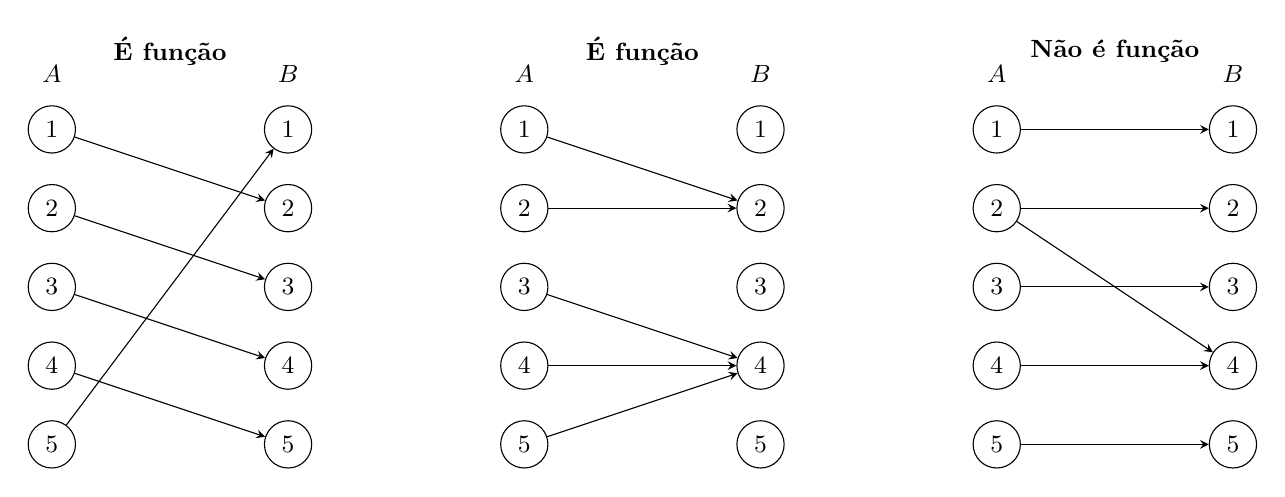
\begin{tikzpicture}[
        every node/.style={font=\small},
        ponto/.style={circle, draw, minimum size=6mm, inner sep=0pt},
        >=stealth
    ]

        %--------------------------------
        % (a) É função
        %--------------------------------
        \node at (1.5,1) {\textbf{É função}};
        \node at (0,0.7) {$A$};
        \node at (3,0.7) {$B$};

        \foreach \y/\v in {0/1,-1/2,-2/3,-3/4,-4/5}
            \node[ponto] (a\v) at (0,\y) {\v};

        \foreach \y/\v in {0/1,-1/2,-2/3,-3/4,-4/5}
            \node[ponto] (b\v) at (3,\y) {\v};

        \draw[->] (a1) -- (b2);
        \draw[->] (a2) -- (b3);
        \draw[->] (a3) -- (b4);
        \draw[->] (a4) -- (b5);
        \draw[->] (a5) -- (b1);


        %--------------------------------
        % (b) É função
        %--------------------------------
        \begin{scope}[xshift=6cm]

            \node at (1.5,1) {\textbf{É função}};
            \node at (0,0.7) {$A$};
            \node at (3,0.7) {$B$};

            \foreach \y/\v in {0/1,-1/2,-2/3,-3/4,-4/5}
                \node[ponto] (c\v) at (0,\y) {\v};

            \foreach \y/\v in {0/1,-1/2,-2/3,-3/4,-4/5}
                \node[ponto] (d\v) at (3,\y) {\v};

            \draw[->] (c1) -- (d2);
            \draw[->] (c2) -- (d2);
            \draw[->] (c3) -- (d4);
            \draw[->] (c4) -- (d4);
            \draw[->] (c5) -- (d4);

        \end{scope}


        %--------------------------------
        % (c) Não é função
        %--------------------------------
        \begin{scope}[xshift=12cm]

            \node at (1.5,1) {\textbf{Não é função}};
            \node at (0,0.7) {$A$};
            \node at (3,0.7) {$B$};

            \foreach \y/\v in {0/1,-1/2,-2/3,-3/4,-4/5}
                \node[ponto] (e\v) at (0,\y) {\v};

            \foreach \y/\v in {0/1,-1/2,-2/3,-3/4,-4/5}
                \node[ponto] (f\v) at (3,\y) {\v};

            \draw[->] (e1) -- (f1);
            \draw[->] (e2) -- (f2);
            \draw[->] (e2) -- (f4);
            \draw[->] (e3) -- (f3);
            \draw[->] (e4) -- (f4);
            \draw[->] (e5) -- (f5);

        \end{scope}

    \end{tikzpicture}
    \caption{Exemplos de relações entre os conjuntos $A$ e $B$. Nos dois primeiros casos, cada elemento de $A$ está associado a um único elemento de $B$, caracterizando uma função. No último caso, o elemento $2\in A$ está associado a dois elementos distintos de $B$ e, portanto, a relação não é uma função.}
    \label{fig:diagramas-funcao}
\end{figure}

\subsection{Domínio de uma função}

Considere uma função $f:A\longrightarrow B$. Chamamos de \textbf{domínio} de $f$, denotado por $D(f)$, o conjunto formado por todos os valores de $x$ para os quais a função está definida. Quando uma função é apresentada apenas por meio de sua expressão algébrica, devemos determinar quais valores de $x$ tornam essa expressão bem definida.

\begin{figure}[H]
    \centering
    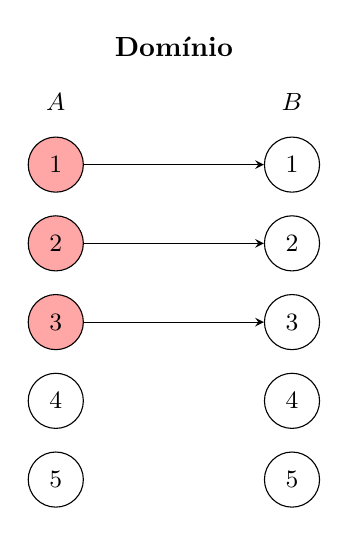
\begin{tikzpicture}[
        >=stealth,
        ponto/.style={circle, draw, minimum size=7mm, inner sep=0pt},
        selecionado/.style={circle, draw, fill=red!35, minimum size=7mm, inner sep=0pt},
        every node/.style={font=\small}
    ]

        % ==================================================
        % DOMÍNIO
        % ==================================================

        \node[font=\bfseries] at (1.5,2) {Domínio};

        \node at (0,1.3) {$A$};
        \node at (3,1.3) {$B$};

        % Elementos de A
        \node[selecionado] (a1) at (0,0.5) {$1$};
        \node[selecionado] (a2) at (0,-0.5) {$2$};
        \node[selecionado] (a3) at (0,-1.5) {$3$};
        \node[ponto]       (a4) at (0,-2.5) {$4$};
        \node[ponto]       (a5) at (0,-3.5) {$5$};

        % Elementos de B
        \node[ponto] (b1) at (3,0.5) {$1$};
        \node[ponto] (b2) at (3,-0.5) {$2$};
        \node[ponto] (b3) at (3,-1.5) {$3$};
        \node[ponto] (b4) at (3,-2.5) {$4$};
        \node[ponto] (b5) at (3,-3.5) {$5$};

        % Setas
        \draw[->] (a1) -- (b1);
        \draw[->] (a2) -- (b2);
        \draw[->] (a3) -- (b3);
    \end{tikzpicture}

    \caption{Representação do domínio e da imagem de uma relação. As bolinhas destacadas em vermelho representam os elementos que pertencem ao domínio, as que não estão em vermelho são pertencem ao conjunto A, porém não ao domínio.}
\end{figure}

Em particular, devemos observar algumas restrições importantes, que em geral são as que aparecem em problemas.

\begin{enumerate}
    \item[(i)] Denominadores não podem ser iguais a zero;
    \item[(ii)] Raízes de índice par não podem possuir radicando negativo, quando trabalhamos no conjunto dos números reais.
\end{enumerate}

\begin{example}
    Considere a função
    \begin{equation}
        f(x)=\frac{1}{x-1}.
    \end{equation}
    Para que a função esteja definida, devemos ter
    \begin{align*}
        x-1 &\neq 0 \\
        x &\neq 1.
    \end{align*}
    Portanto,
    \begin{equation}
        D(f)=\{x\in\mathbb{R}:x\neq1\}
        =\mathbb{R}\setminus\{1\}.
    \end{equation}

    Por exemplo,
    \begin{align*}
        f(2)&=\frac{1}{2-1}=1,
        &
        f(3)&=\frac{1}{3-1}=\frac{1}{2}.
    \end{align*}
\end{example}

\begin{example}
    Considere a função
    \begin{equation}
        f(x)=\sqrt{2x-4}.
    \end{equation}
    Como estamos trabalhando em $\mathbb{R}$, devemos ter
    \begin{align*}
        2x-4 &\geq 0 \\
        2x &\geq 4 \\
        x &\geq 2.
    \end{align*}
    Portanto,
    \begin{equation*}
        D(f)=\{x\in\mathbb{R}:x\geq2\}=[2,\infty).
    \end{equation*}
\end{example}

\subsection{Conjunto Imagem}

Considere novamente uma função $f:A\to B$. Chamamos de \textbf{imagem} de $f$, denotada por $\operatorname{Im}(f)$, o conjunto formado pelos elementos de $B$ que estão associados a pelo menos um elemento do domínio.

Formalmente,
\begin{equation}
    \operatorname{Im}(f)
    =\{y\in B:\text{ existe }x\in A\text{ tal que }y=f(x)\}.
\end{equation}

Observe que a imagem de uma função é sempre um subconjunto de seu contradomínio, isto é,
\begin{equation}
    \operatorname{Im}(f)\subseteq B.
\end{equation}

\begin{figure}[H]
    \centering
    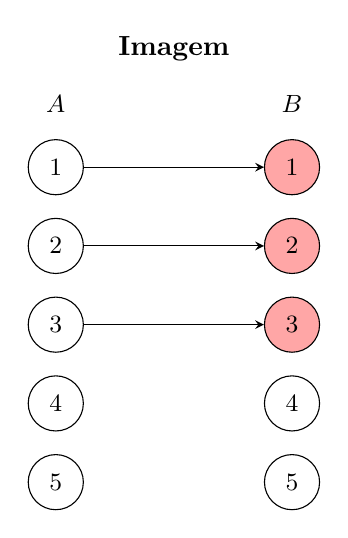
\begin{tikzpicture}[
        >=stealth,
        ponto/.style={circle, draw, minimum size=7mm, inner sep=0pt},
        selecionado/.style={circle, draw, fill=red!35, minimum size=7mm, inner sep=0pt},
        every node/.style={font=\small}
    ]

       


        % ==================================================
        % IMAGEM
        % ==================================================

        \begin{scope}[xshift=7cm]

            \node[font=\bfseries] at (1.5,2) {Imagem};

            \node at (0,1.3) {$A$};
            \node at (3,1.3) {$B$};

            % Elementos de A
            \node[ponto] (c1) at (0,0.5) {$1$};
            \node[ponto] (c2) at (0,-0.5) {$2$};
            \node[ponto] (c3) at (0,-1.5) {$3$};
            \node[ponto] (c4) at (0,-2.5) {$4$};
            \node[ponto] (c5) at (0,-3.5) {$5$};

            % Elementos de B
            \node[selecionado] (d1) at (3,0.5) {$1$};
            \node[selecionado] (d2) at (3,-0.5) {$2$};
            \node[selecionado] (d3) at (3,-1.5) {$3$};
            \node[ponto]       (d4) at (3,-2.5) {$4$};
            \node[ponto]       (d5) at (3,-3.5) {$5$};

            % Setas
            \draw[->] (c1) -- (d1);
            \draw[->] (c2) -- (d2);
            \draw[->] (c3) -- (d3);

        \end{scope}

    \end{tikzpicture}

    \caption{Representação do domínio e da imagem de uma relação. As bolinhas destacadas em vermelho representam os elementos que pertencem ao domínio, à esquerda, e à imagem, à direita.}
\end{figure}


\begin{example}
    Considere a função
    \begin{equation}
        f:\mathbb{R}\longrightarrow\mathbb{R},
        \qquad
        f(x)=x^2-1.
    \end{equation}
    Como $x^2\geq0$ para todo $x\in\mathbb{R}$, temos
    \begin{equation}
        x^2-1\geq-1.
    \end{equation}
    Além disso, todo valor real maior ou igual a $-1$ pode ser obtido pela função. Portanto,
    \begin{equation}
        \operatorname{Im}(f)
        =\{y\in\mathbb{R}:y\geq-1\}
        =[-1,\infty).
    \end{equation}
\end{example}

Uma função é caracterizada por três elementos fundamentais
\begin{enumerate}
    \item seu \textbf{domínio};
    \item seu \textbf{contradomínio};
    \item sua \textbf{lei de formação}, isto é, a regra que determina $f(x)$ para cada $x$ pertencente ao domínio.
\end{enumerate}

Assim, ao escrevermos
\begin{equation}
    f:A\longrightarrow B,
    \qquad
    x\longmapsto f(x),
\end{equation}
estamos especificando o domínio $A$, o contradomínio $B$ e a regra que associa cada $x\in A$ ao seu respectivo valor $f(x)\in B$.

\subsection{Gráfico}

Considere uma função $f:A\to B$. Chamamos de \textbf{gráfico de $f$} o conjunto de todos os pares ordenados $(x,f(x))$, com $x\in A$. Isto é,
\begin{equation*}
    G(f)=\{(x,f(x)):x\in A\}.
\end{equation*}

Geometricamente, quando $A$ e $B$ são subconjuntos de $\mathbb{R}$, cada par $(x,f(x))$ pode ser representado como um ponto no plano cartesiano. O conjunto de todos esses pontos constitui a representação gráfica da função.

Observe que, para cada valor $x$ pertencente ao domínio, existe um único valor $f(x)$ associado. Consequentemente, uma reta vertical não pode intersectar o gráfico de uma função em mais de um ponto. Essa observação é conhecida como \textbf{teste da reta vertical}.

\begin{figure}[H]
    \centering
    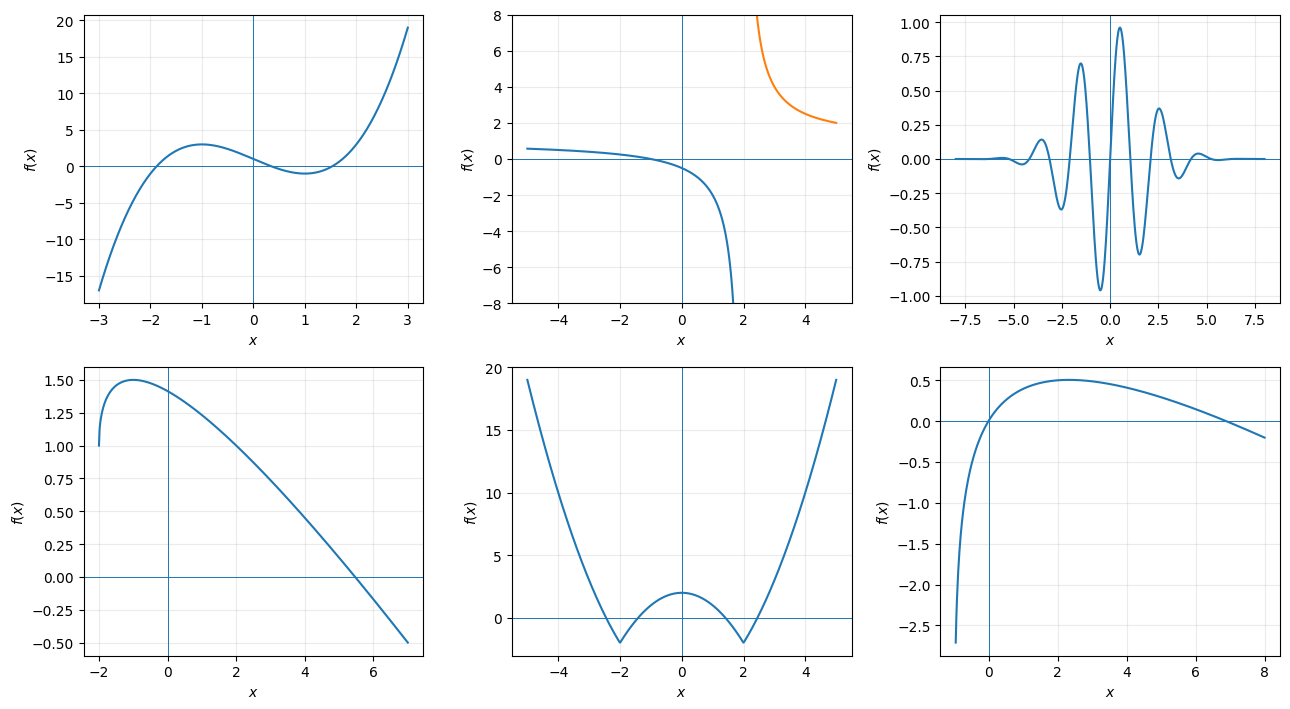
\includegraphics[width=\textwidth]{figuras/graficos_funcoes_3x2.png}
    \caption{Exemplos de representações gráficas de diferentes funções reais. Cada ponto do gráfico possui a forma $(x,f(x))$, em que $x$ pertence ao domínio da respectiva função.}
    \label{fig:exemplos-graficos-funcoes}
\end{figure}

\section{Função afim}

Até o momento, estudamos funções de maneira geral, apresentando conceitos como domínio, contradomínio, imagem e representação gráfica. A partir de agora, começaremos a afunilar nosso estudo, considerando algumas classes particulares de funções que aparecem com frequência tanto na Matemática quanto na modelagem de fenômenos reais.

Uma das classes mais simples e importantes é a das \textbf{funções afins}. Diversos fenômenos podem ser modelados, ao menos aproximadamente, por meio de uma função afim. Além de sua simplicidade matemática, um dos principais motivos para o interesse nesse tipo de modelo é sua fácil interpretabilidade, uma vez que seus parâmetros possuem significados claros e permitem compreender diretamente como uma variável se modifica em função de outra.



\begin{defin}
    Chamamos de \textbf{função afim} toda função $f:\mathbb{R}\to\mathbb{R}$ que pode ser escrita na forma
\begin{equation*}
    f(x)=ax+b,
\end{equation*}
em que $a,b\in\mathbb{R}$ são constantes.
\end{defin}

\begin{figure}[H]
    \centering
    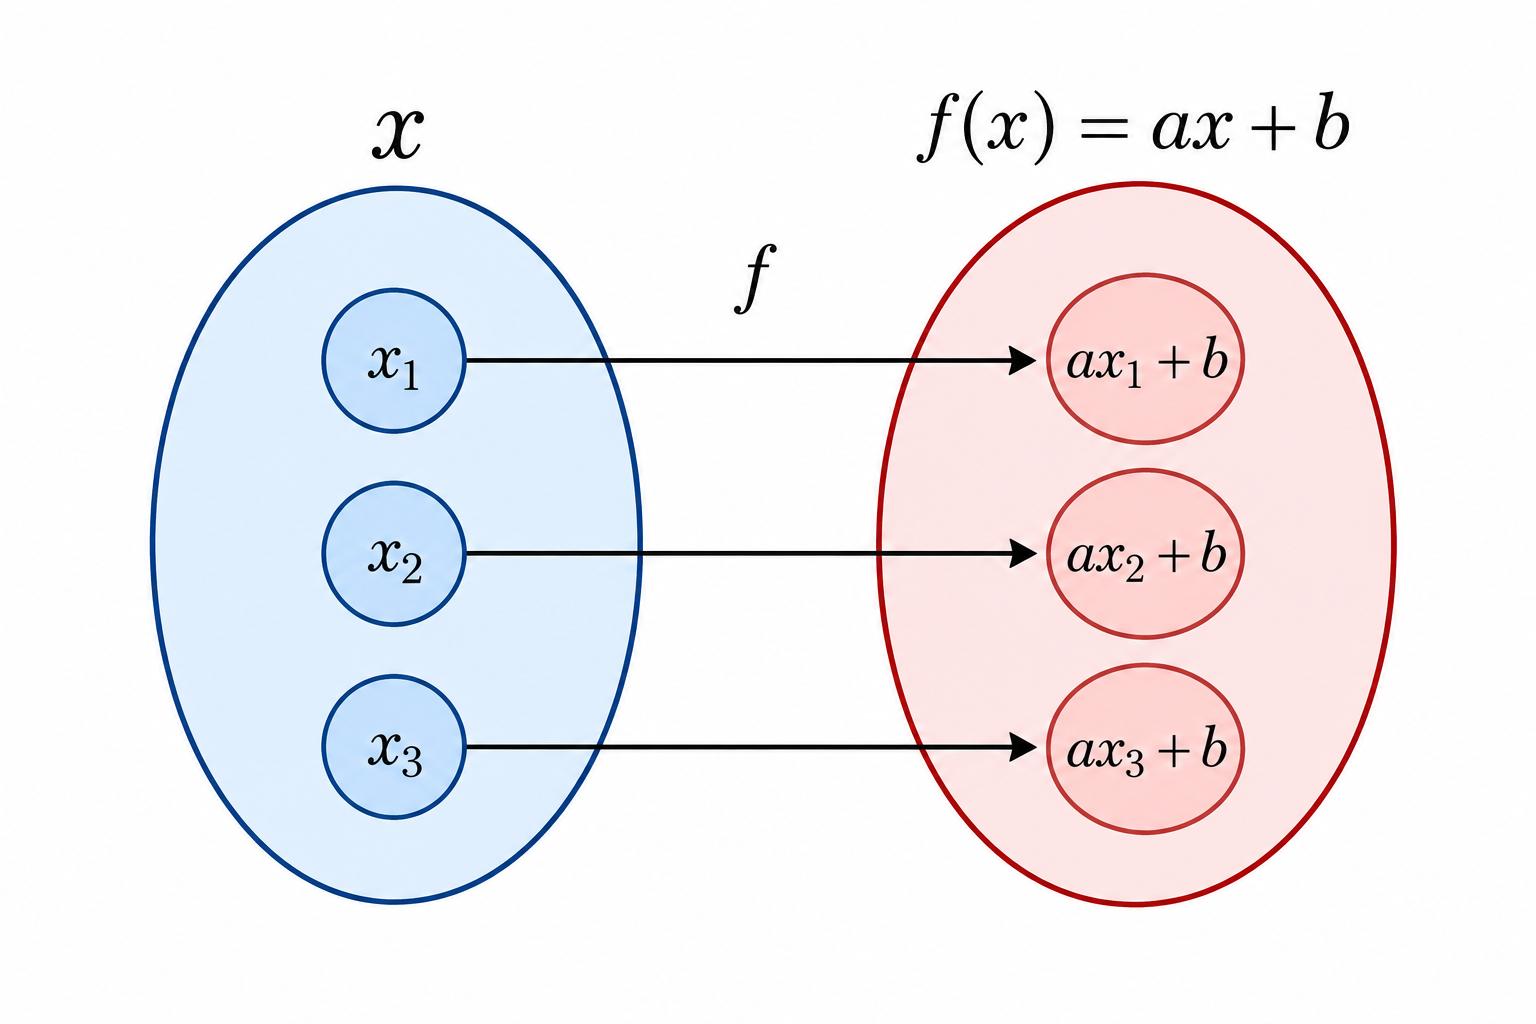
\includegraphics[width=0.8\textwidth]{figuras/diagrama_afim.png}
    \caption{Representação da função afim $f(x)=ax+b$ por meio de um diagrama.}
    \label{fig:diagrama_afim}
\end{figure}

O parâmetro $a$ é chamado de \textbf{coeficiente angular} e determina a taxa de variação da função. Em outras palavras, ele indica quanto o valor de $f(x)$ varia quando aumentamos $x$ em uma unidade. De fato,
\begin{equation*}
    f(x+1)-f(x)=a.
\end{equation*}
Assim, quando $a>0$, a função cresce à medida que $x$ aumenta; quando $a<0$, a função decresce; e, quando $a=0$, temos uma função constante.

O parâmetro $b$ é chamado de \textbf{coeficiente linear} e representa o valor assumido pela função quando $x=0$. De fato,
\begin{equation*}
    f(0)=a\cdot0+b=b.
\end{equation*}

Dessa forma, os dois parâmetros possuem interpretações bastante naturais: enquanto $a$ descreve a \textbf{taxa de variação} da função, $b$ determina seu \textbf{valor inicial}, isto é, o valor da função quando $x=0$.

\begin{example}
    Considere a função afim
    \begin{equation*}
        f(x)=2x+3.
    \end{equation*}
    Podemos estar interessados tanto em determinar a imagem de um determinado valor de $x$ quanto em realizar o processo inverso, isto é, determinar qual valor de $x$ possui uma imagem previamente especificada.

    Por exemplo, para determinar a imagem de $x=1$, basta substituir esse valor na função:
    \begin{align*}
        f(1)&=2\cdot1+3=5.
    \end{align*}
    Portanto, a imagem de $1$ pela função $f$ é $5$.

    Agora, suponha que desejamos determinar qual valor de $x$ possui imagem igual a $10$. Nesse caso, procuramos $x$ tal que $f(x)=10$. Assim,
    \begin{align*}
        2x+3&=10 \\
        2x&=7 \\
        x&=\frac{7}{2}.
    \end{align*}
    Portanto,
    \begin{equation*}
        f\left(\frac{7}{2}\right)=10.
    \end{equation*}

    Dessa forma, quando conhecemos $x$, podemos calcular diretamente sua imagem $f(x)$. Por outro lado, quando conhecemos o valor da imagem, podemos determinar o valor de $x$ correspondente resolvendo a equação $f(x)=y$.
\end{example}


Geometricamente, portanto, $b$ determina o ponto em que o gráfico da função intersecta o eixo vertical. Agora provaremos no Teorema~\ref{reta}  que o gráfico da função afim é dado por uma reta. 

\begin{teo}
\label{reta}
    Seja $f:\mathbb{R}\to\mathbb{R}$ uma função afim dada por $f(x)=ax+b$, com $a,b\in\mathbb{R}$. Então o gráfico de $f$ é uma reta no plano cartesiano.
\end{teo}

\begin{proof}
    Considere dois pontos distintos do gráfico de $f$,
    \begin{equation*}
        P_1=(x_1,f(x_1))
        \qquad\text{e}\qquad
        P_2=(x_2,f(x_2)),
    \end{equation*}
    com $x_1\neq x_2$. O coeficiente angular da reta que passa por esses dois pontos é dado por
    \begin{align*}
        \frac{f(x_2)-f(x_1)}{x_2-x_1}
        &=\frac{(ax_2+b)-(ax_1+b)}{x_2-x_1}
        =\frac{a(x_2-x_1)}{x_2-x_1}
        =a.
    \end{align*}
    Portanto, quaisquer dois pontos distintos do gráfico determinam sempre o mesmo coeficiente angular $a$. Além disso, como
    \begin{equation*}
        f(0)=b,
    \end{equation*}
    o gráfico passa pelo ponto $(0,b)$. Consequentemente, todos os pontos $(x,f(x))$ satisfazem a equação
    \begin{equation*}
        y=ax+b,
    \end{equation*}
    que é a equação de uma reta de coeficiente angular $a$ e que intersecta o eixo vertical no ponto $(0,b)$. Logo, o gráfico de $f$ é uma reta.
\end{proof}
A Figura~\ref{fig:grade_funcoes_afins} mostra vários comportamentos da reta da função $f(x) = ax+b$ 

\begin{figure}[H]
    \centering
    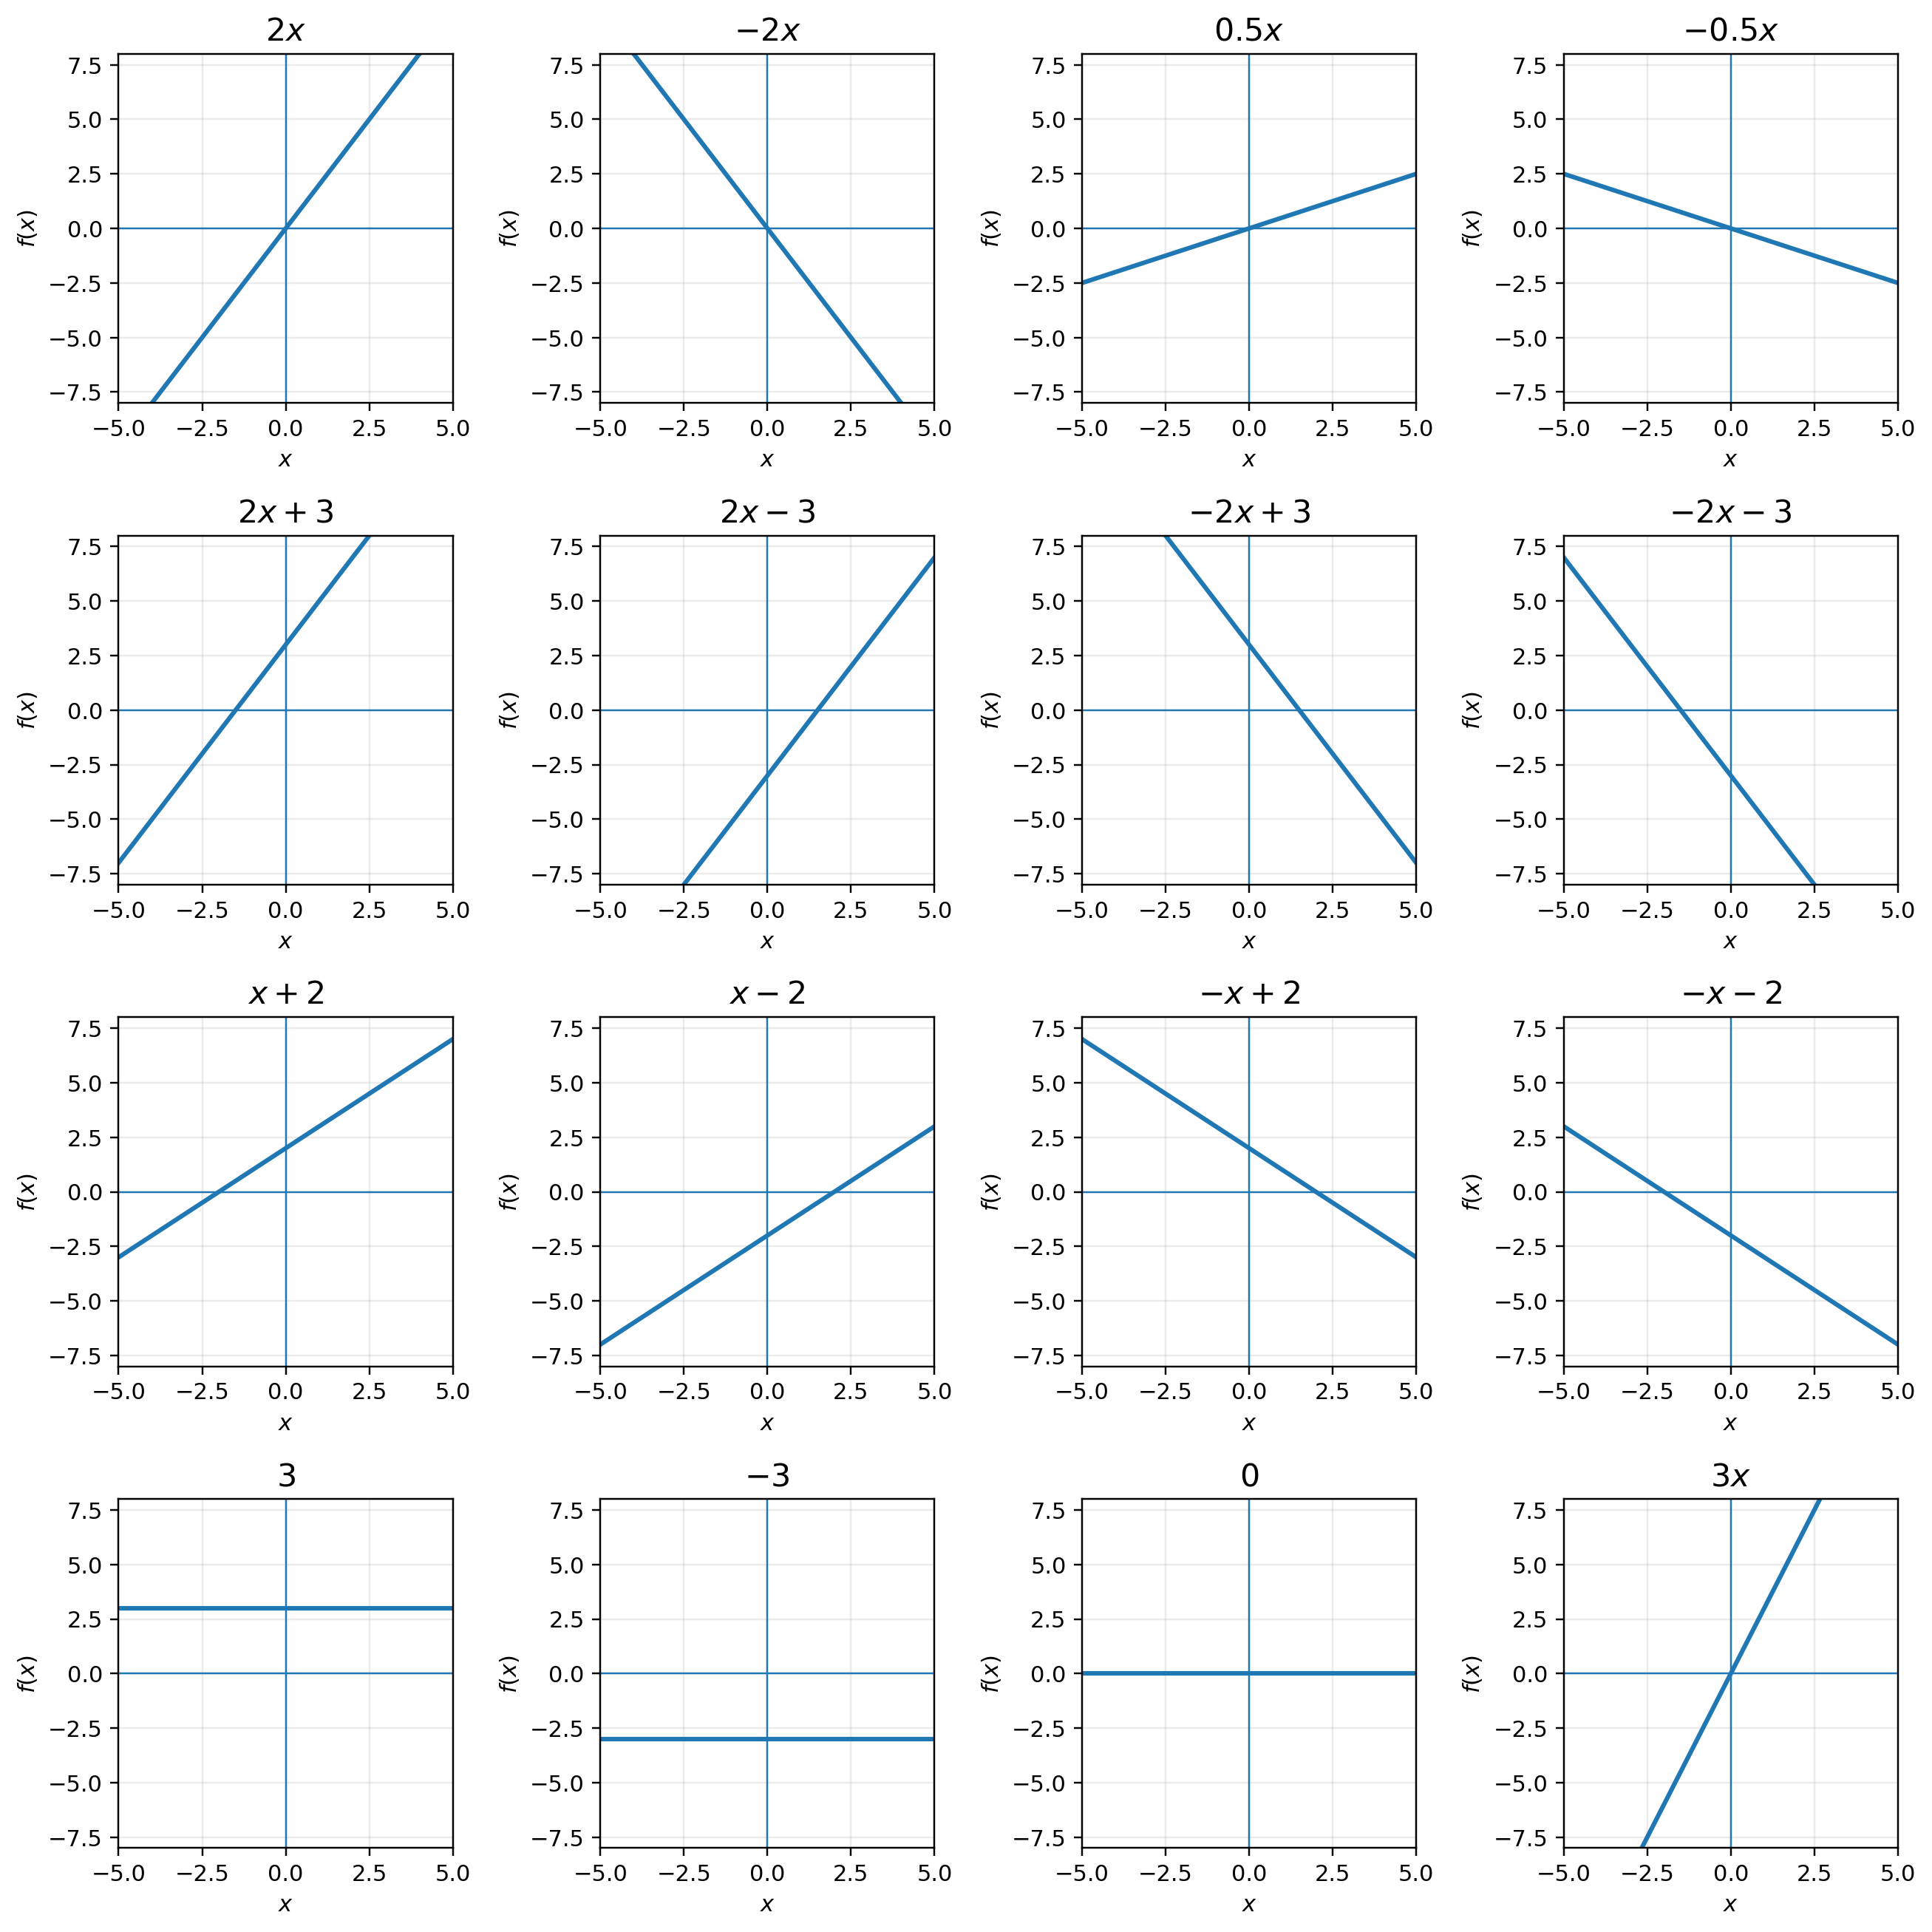
\includegraphics[width=0.79\textwidth]{figuras/grade_funcoes_afins_4x4.png}
    \caption{Exemplos de gráficos de funções afins para diferentes valores dos coeficientes $a$ e $b$.}
    \label{fig:grade_funcoes_afins}
\end{figure}

\subsection{Aplicações da função afim}

A função afim pode ser utilizada para representar situações nas quais uma quantidade varia a uma taxa constante em relação a outra. Nesses casos, o coeficiente angular $a$ representa justamente essa taxa de variação, enquanto o coeficiente linear $b$ representa o valor inicial da quantidade estudada. Vejamos alguns exemplos.

\begin{example}
    Considere uma obra na qual a utilização de concreto envolve um custo fixo de R\$ $1.200,00$, referente à mobilização dos equipamentos, além de um custo de R\$ $450,00$ para cada metro cúbico de concreto utilizado.

    Se $x$ representa o volume de concreto utilizado, em metros cúbicos, e $C(x)$ representa o custo total, podemos organizar alguns valores na seguinte tabela:

    \begin{center}
        \begin{tabular}{c|c}
            \hline
            Volume ($\text{m}^3$) & Custo (R\$) \\
            \hline
            0  & $1.200$ \\
            2  & $2.100$ \\
            4  & $3.000$ \\
            6  & $3.900$ \\
            8  & $4.800$ \\
            10 & $5.700$ \\
            \hline
        \end{tabular}
    \end{center}

    Observe que, a cada aumento de $1\,\text{m}^3$ no volume de concreto, o custo aumenta R\$ $450,00$. Além disso, quando $x=0$, ainda existe o custo fixo de R\$ $1.200,00$. Dessa forma, o modelo algébrico é dado por
    \begin{equation*}
        C(x)=450x+1200.
    \end{equation*}

    Nesse modelo, $a=450$ representa o custo adicional por metro cúbico de concreto, enquanto $b=1200$ representa o custo inicial da operação.

    \begin{figure}[H]
        \centering
        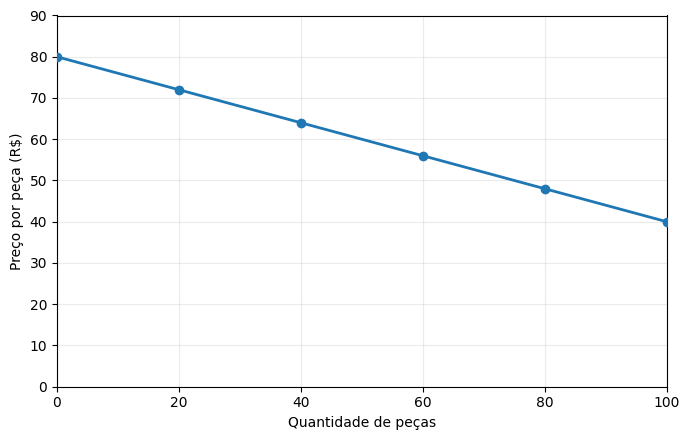
\includegraphics[width=0.7\textwidth]{figuras/exemplo_afim_civil.png}
        \caption{Custo em função do volume de concreto utilizado.}
        \label{fig:afim_engenharia}
    \end{figure}
\end{example}

\begin{example}
    Considere um modelo simplificado para representar a energia disponível de um jogador durante uma partida de futebol. Suponha que o jogador inicie a partida com $100\%$ de energia disponível e que, segundo o modelo, esse percentual diminua $0{,}6$ ponto percentual a cada minuto de jogo.

    Se $t$ representa o tempo de jogo, em minutos, e $E(t)$ representa o percentual de energia disponível, temos:

    \begin{center}
        \begin{tabular}{c|c}
            \hline
            Tempo (min) & Energia disponível (\%) \\
            \hline
            0  & $100$ \\
            15 & $91$ \\
            30 & $82$ \\
            45 & $73$ \\
            60 & $64$ \\
            75 & $55$ \\
            90 & $46$ \\
            \hline
        \end{tabular}
    \end{center}

    Como a energia diminui $0{,}6$ ponto percentual por minuto, temos $a=-0{,}6$. Além disso, no instante inicial, $E(0)=100$. Portanto, o modelo é
    \begin{equation*}
        E(t)=-0{,}6t+100.
    \end{equation*}

    Nesse exemplo, o coeficiente negativo indica que a variável estudada diminui com o passar do tempo. O coeficiente $b=100$, por sua vez, representa a energia disponível no início da partida.

    \begin{figure}[H]
        \centering
        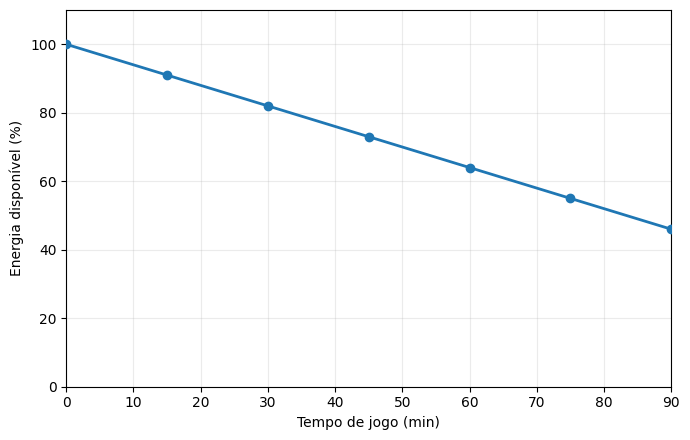
\includegraphics[width=0.7\textwidth]{figuras/exemplo_afim_futebol.png}
        \caption{Modelo simplificado da energia disponível de um jogador em função do tempo de jogo.}
        \label{fig:afim_futebol}
    \end{figure}
\end{example}

\begin{example}
    Considere uma confecção que estabelece o preço por peça de determinado produto de acordo com a quantidade encomendada. Suponha que o preço inicial seja de R\$ $80,00$ por peça e que, em uma determinada faixa de produção, a empresa conceda um desconto de R\$ $0,40$ no preço unitário para cada unidade acrescentada ao pedido.

    Se $q$ representa a quantidade de peças e $P(q)$ representa o preço unitário, alguns valores desse modelo são:

    \begin{center}
        \begin{tabular}{c|c}
            \hline
            Quantidade de peças & Preço por peça (R\$) \\
            \hline
            0   & $80$ \\
            20  & $72$ \\
            40  & $64$ \\
            60  & $56$ \\
            80  & $48$ \\
            100 & $40$ \\
            \hline
        \end{tabular}
    \end{center}

    Nesse caso, cada unidade adicional reduz o preço unitário em R\$ $0,40$. Logo, a taxa de variação é $a=-0{,}4$. Como o valor inicial utilizado pelo modelo é $b=80$, obtemos
    \begin{equation*}
        P(q)=-0{,}4q+80.
    \end{equation*}

    Novamente, o sinal negativo do coeficiente angular indica uma relação decrescente: quanto maior a quantidade encomendada, menor é o preço por peça, dentro da faixa em que o modelo é considerado válido.

    \begin{figure}[H]
        \centering
        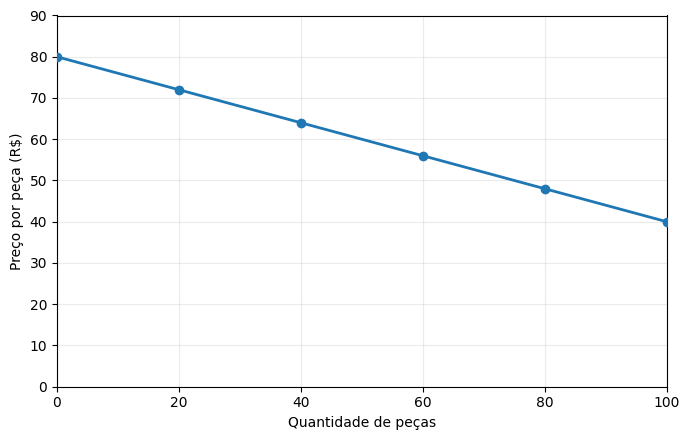
\includegraphics[width=0.7\textwidth]{figuras/exemplo_afim_moda.png}
        \caption{Preço unitário em função da quantidade de peças encomendadas.}
        \label{fig:afim_moda}
    \end{figure}
\end{example}



